%!TEX root = ../template.tex
%%%%%%%%%%%%%%%%%%%%%%%%%%%%%%%%%%%%%%%%%%%%%%%%%%%%%%%%%%%%%%%%%%%%
%% chapter4.tex
%% NOVA thesis document file
%%
%% Chapter with lots of dummy text
%%%%%%%%%%%%%%%%%%%%%%%%%%%%%%%%%%%%%%%%%%%%%%%%%%%%%%%%%%%%%%%%%%%%

\typeout{NT FILE chapter4.tex}%

\chapter{Dimensional Inspection and Measurement Equipment}
\label{cha:lorem_ipsum}

This chapter introduces the equipment and methodology that can be used for dimensional inspection in engine component analysis. Keeping parts within the required tolerances is essential for ensuring performance and durability. A 3D scanner makes it possible to generate a digital model of the components, while a coordinate measuring machine (CMM) allows for precise measurement and comparison with nominal dimensions. These tools help improve the accuracy of the analysis and support potential optimization of the components at \gls{TAP} \gls{ME} Engine Shop.

The Engine Shop at \gls{TAP} \gls{ME} has a specialized Dimensional Inspection department responsible for verifying component dimensions in accordance with the manual, ensuring optimal engine performance and reliability.

\section{Available Measurement Equipment}
\label{sec:equipment}

To ensure precise measurements, the department relies on advanced equipment, such as the Creaform HandySCAN 3D scanner, which captures highly accurate digital models of components, and the Mitutoyo Euro-C 121210 coordinate measuring machine (CMM), which provides detailed dimensional and geometric analysis. By using these tools, the team can carry out thorough inspections, verify tolerances, and explore opportunities for improving component performance.

\subsection{Creaform HandySCAN 3D scanner}
\label{sec:scanner}

The HandySCAN 3D is a high-precision laser scanner developed by Creaform, designed for portable 3D scanning of objects with complex geometries. It uses laser triangulation to capture detailed 3D models with high accuracy and resolution.
It presents the following technical data: 
\begin{itemize}
    \item \textbf{Accuracy}: 0.025 mm (0.0009 in)
    \item \textbf{Volumetric Accuracy}: Up to 0.020 mm + 0.015 mm/m
    \item \textbf{Light Source}: 22–30 blue laser lines
    \item \textbf{Working Distance}: 200 to 750 mm
    \item \textbf{Recommended Part Size Range}: 0.05 – 4 m
    \item \textbf{Weight}: 0.94 kg
\end{itemize}

The HandySCAN 3D laser scanner is used in conjunction with VXelements, an integrated 3D software platform that allos real-time data acquisition, post-processing, and analysis.

During the development of this thesis, this equipment will enable the practice of reverse engineering. Using the HandySCAN 3D scanner, detailed physical data from the \gls{HPC} blades can be captured, and with the VXelements software, the point cloud is transformed into a 3D \gls{CAD} model. This model can then be imported into SolidWorks for further analysis and used to design the workpiece, which will be employed in the \gls{CMM} to securely hold the blades during measurement.

\subsection{Mitutoyo Euro-C 121210}
\label{sec:cmm}

The \gls{CMM} is a highly precise tool used to measure the geometry of parts and components. It works by using a probe that senses the physical contact with the object. While traditional CMMs rely on touch-trigger probes, there are other models that use laser or optical sensors to take measurements. The Mitutoyo Euro-C 121210 \gls{CMM} is controlled by a computer and operates within a three-dimensional coordinate system.

This particular CMM is equipped with a Renishaw Revo-2, providing it with five degrees of freedom (DoF). In addition to moving along the three main axes, the machine can adjust the probe’s angles, enabling it to measure even the most complex surfaces that would otherwise be difficult to reach. The machine setup includes a granite bed, probe, probe tree, arm, joystick, and specialized software, as shown in Figure~\ref{fig:cmm}.

Although four probes are available for use with the Renishaw Revo-2, only two are applicable to this project. Among them, the RSP2-3 is the sole probe that enables full five-degree-of-freedom operation. As illustrated in Figure~\ref{fig:dof}, the first three DoFs (X, Y, and Z) are controlled by the \gls{CMM} arm, while the remaining two ($\alpha$, $\beta$) are executed by the probe itself.

Each probe has distinct characteristics suited for different tasks, as detailed in Table~\ref{tab:probes}.


\begin{table}[ht]
    \caption{Renishaw probes available at TAP}
    \label{tab:probes}
    \centering
    \begin{tabular}{cccc}
    \toprule
    \textbf{Probe} & DoF & Scanning Capability & Sphere $\varnothing$ \\ \hline
    \textbf{RSP2-3} &  5 & 2D & 6mm \\ \hline
    \textbf{RSP3}  & 3 & 3D & 4mm \\ \hline
\end{tabular}
\end{table} 

\begin{figure}[H]
    \centering
    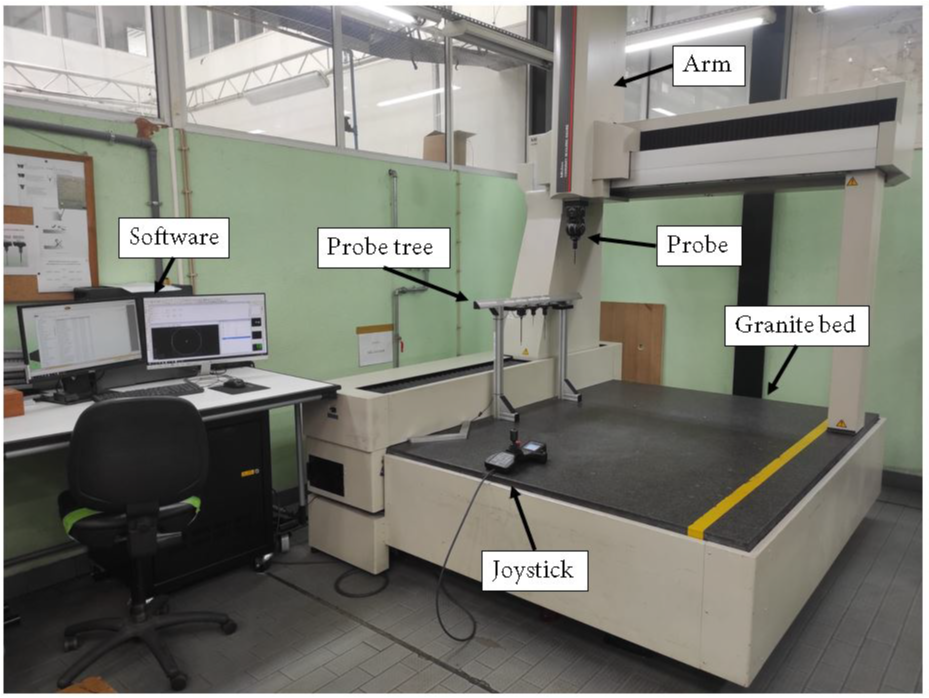
\includegraphics[width=0.8\textwidth]{cmm}
    \caption{Mitutoyo Euro-C 121210 Components \cite{Shi2023}}
    \label{fig:cmm}
\end{figure}

\begin{figure}[H]
    \centering
    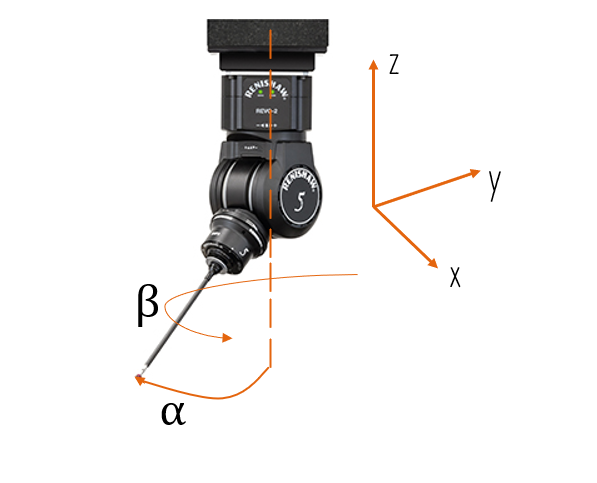
\includegraphics[width=0.4\textwidth]{dof}
    \caption{DOF of the Renishaw probe \cite{renishaw2025}}
    \label{fig:dof}
\end{figure}

The integration of the \gls{CMM} into this project plays a key role in ensuring that every high-pressure compressor rotor blade is measured quickly, accurately, and consistently. The development of a custom inspection program aims to enable the production team to measure entire sets of blades with minimal manual intervention, enhancing both efficiency and reliability.

Through the use of the \gls{CMM}, it is possible to automatically verify critical dimensions, such as \gls{CL}, \gls{LET}, \gls{TET}, and overall airfoil geometry. This ensures that each blade meets the required tolerances while eliminating inconsistencies associated with manual measurement methods. Additionally, this automation reduces the workload of operators, allowing them to focus on other essential tasks while the machine performs the measurements.

Another significant advantage of the \gls{CMM} is its ability to generate detailed inspection reports, facilitating the tracking of blade conditions over time. This capability extends beyond simple compliance verification, contributing to predictive maintenance strategies that enhance engine performance and reduce unexpected maintenance costs.

By incorporating this level of automation and precision into the inspection process, the proposed approach aims to streamline production, improve quality control, and establish a more efficient and standardized methodology for \gls{TAP}’s maintenance operations.

\section{TAP ME: Previous Theses on Dimensional Inspection}
\label{sec:before}

In the past, several master's theses have been developed in collaboration with \gls{TAP} \gls{ME}, contributing to the improvement of measurement and inspection processes for aircraft engine components. One of these studies was conducted by Farinha, E. \cite{Farinha2021}, focusing on the design of a fixture and the development of a measurement method for high-pressure compressor (HPC) rotor blades. This research continued the work initiated by Rendas, P. [13], who laid the foundation for the development of a fixture specifically designed for HPC rotor blade inspection.

Additionally, Baptista, F. \cite{rendas2021fixture} contributed to this field by developing a model that predicts the off-design performance of the CFM56-5B turbofan engine. More recently, Guerreiro, A. \cite{guerreiro} worked on the development of a process to measure the exit flow area of the low-pressure turbine (LPT) nozzles from the same engine model. His study focused on creating an automated program for Coordinate Measuring Machine (CMM) inspection, addressing a previously undeveloped process within \gls{TAP} \gls{ME}’s engine maintenance operations.

While previous studies have primarily focused on components of the CFM56-5B engine, this thesis aims to extend the dimensional inspection process to the HPC rotor blades of the LEAP-1A engine. One project involves developing an optimized CMM measurement program for assessing the blade chord to evaluate performance, utilizing data from the test bank. The second project focuses on measuring and controlling platform clearance to optimize the assembly process. These improvements, applied to both the LEAP and CFM engines, build on previous research, further advancing the continuous optimization of inspection methods to adapt to newer engine generations.


\chapter{Current Progress and Work Plan}
\label{cha:planeamento}

The analysis of the operation of the Maintenance and Engineering Unit included a demonstration of the component scanning process and a session on the functionality of the \gls{CMM}. Following this, the process through which blades go through maintenance was described in detail, as shown in Figure~\ref{fig:esquema}, outlining each step in the maintenance cycle.

Additionally, a collection of scrapped \gls{HPC} blades from a \gls{LEAP}-1A engine was carried out, involving the tracking of blades that had been discarded during previous maintenance activities. This collection enabled the scanning and dimensional comparison between a new and a worn blade, with the goal of analyzing the extent of blade degradation over time and understanding its potential impact on performance.

In parallel, work on test cell data analysis was initiated, aiming to develop a program to assess the impact of variations in sensor readings on the final engine \gls{EGT} measurement. This analysis seeks to identify key parameters that influence test cell results and to understand how performance evaluation is carried out. By gaining deeper insights into these factors, it will be possible to facilitate future analyses of the impact of blade chord length variations on engine performance.

\begin{figure}[H]
    \centering
    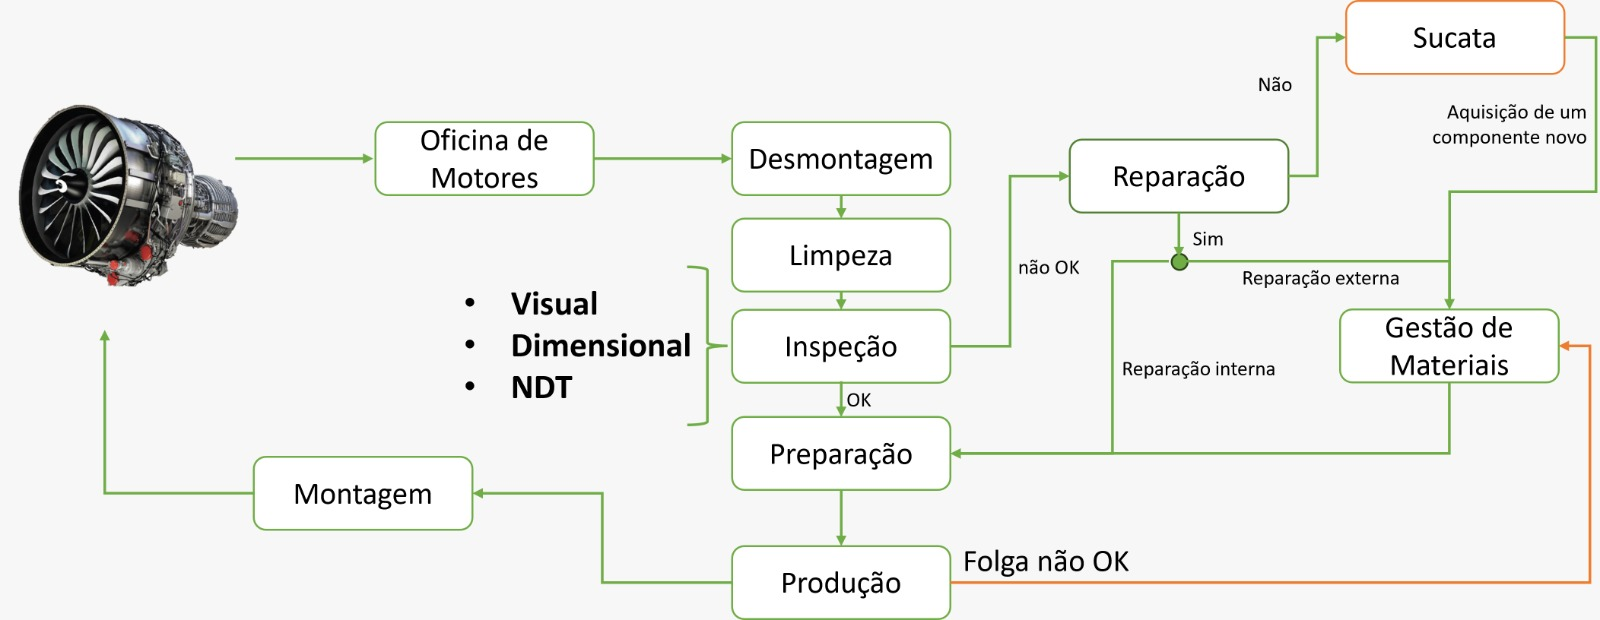
\includegraphics[width=0.8\textwidth]{esquema.jpeg}
    \caption{Process overview of blade maintenance cycle}
    \label{fig:esquema}
\end{figure}

\section{Work Plan}
\label{sec:plano}

To ensure a well-structured and efficient workflow, a provisional task plan has been created, as shown in Figure~\ref{fig:plan_prov}. The schedule will distribute key tasks over the coming months, allowing a balanced approach between research, development, and documentation. The initial phase focused on bibliographic research and drafting the dissertation introduction, providing a solid theoretical foundation. At the same time, work on scan processing and measurement tools will begin, setting the groundwork for later stages. Midway through the project, efforts will shift toward programming for chord measurement and analyzing test bench data—crucial steps for assessing engine performance. The final months will be dedicated to wrapping up the dissertation and completing the internship, ensuring all research components are properly integrated and documented. This structured approach is expected to help develop a project with practical value for the company while providing a highly enriching learning experience for the student.

\begin{figure}[H]
    \centering
    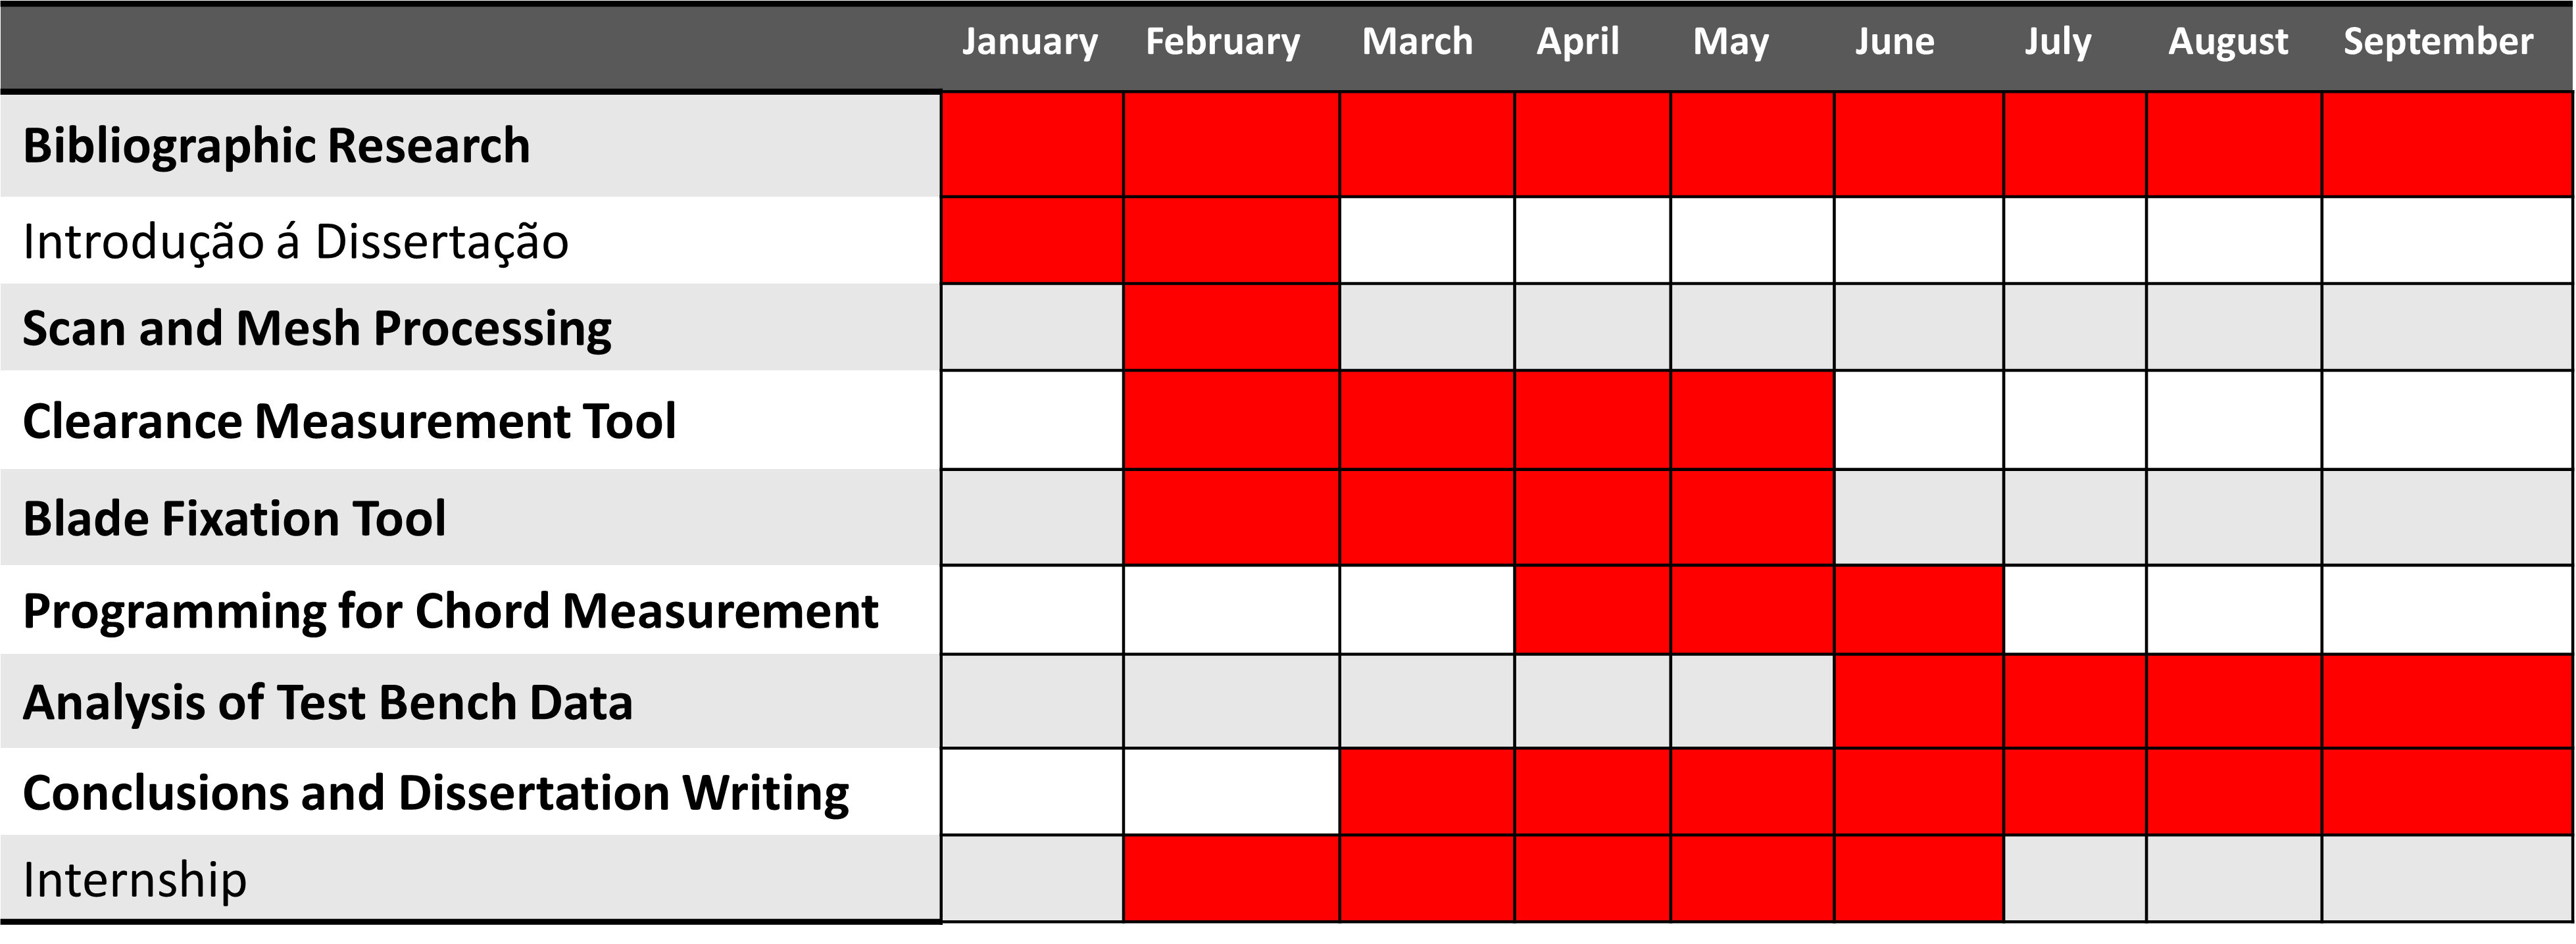
\includegraphics[width=0.8\textwidth]{plan_prov}
    \caption{Work Plan.}
    \label{fig:plan_prov}
\end{figure}



\chapter{Problem Definition and Scope}
\label{cha:definition}

This thesis tackles two key challenges in the assembly of HPC (High Pressure Compressor) blades. The goal is to ensure that the assembly process meets the required specifications and to better understand how blade geometry impacts engine performance.

The first challenge is to develop a process or tool that guarantees the correct assembly clearance for the blades. This clearance must comply with the specifications outlined in the engine manual, ensuring that the blades are assembled properly and function as intended.

The second objective is to create a reliable method for measuring the chord length of the blades and analyzing its correlation with engine performance in bench tests. By understanding this relationship, we can gain valuable insights into how small variations in manufacturing affect overall efficiency and explore ways to optimize the assembly process. Ultimately, this aims to guarantee and control engine performance according to operational needs.

Together, these objectives shape the scope of this work, which involves designing measurement tools, validating methodologies, and bridging the gap between manufacturing precision and engine performance.

In this chapter, the details of these challenges will be explored, along with the initial requirements and decisions that guided the approach taken. This will provide a comprehensive understanding of the context, constraints, and considerations that influenced the development of solutions throughout the project.

\section{Blade Assembly Process and Clearance Requirements}
\label{sec: bladeandclearence}

This study focuses on the assembly of HPC stages 6 to 10, represented in Figure~\ref{fig:hpcass},  as these are the stages that incorporate the blades under analysis, as previously mentioned. The assembly of \gls{HPC} blades follows a standardized procedure to ensure precise positioning and compliance with the required specifications. The process begins with preparing the spool, where blade slots and wire seal grooves are cleaned and inspected. Contaminants are removed to ensure a smooth surface for blade insertion. Wire seals are then installed in the grooves, adhering to specified clearance tolerances to maintain structural integrity.

\begin{figure}[H]
    \centering
    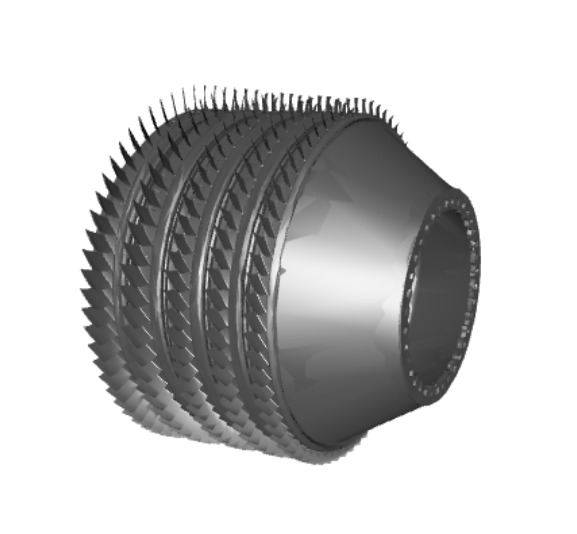
\includegraphics[width=0.5\textwidth]{hpcass.jpeg}
    \caption{\gls{LEAP}-1A \gls{HPC}.}
    \label{fig:hpcass}
\end{figure}


The blades are then inserted into the spool, following a controlled sequence to ensure a uniform distribution. During this step, each blade is checked for free movement within the dovetail slot, as any restrictions may indicate the need for replacement. After all blades are in place, locking blades are installed in designated positions to secure the assembly.

To finalize the assembly, locking lugs are positioned and their set screws are torqued to the required values. A detailed verification is performed to ensure that the locking lugs are correctly engaged within the spool’s dovetail lock slot, preventing unintended movement. To confirm the correct platform clearance, the blades are shifted in one direction to determine the maximum gap, and measurements are taken to verify compliance with the permissible range. This clearance, referred to as Clearance R, is represented in Figure~\ref{fig:assembly6}.If necessary, adjustments are made by replacing narrow-platform blades with wide-platform ones.

\begin{figure}[H]
    \centering
    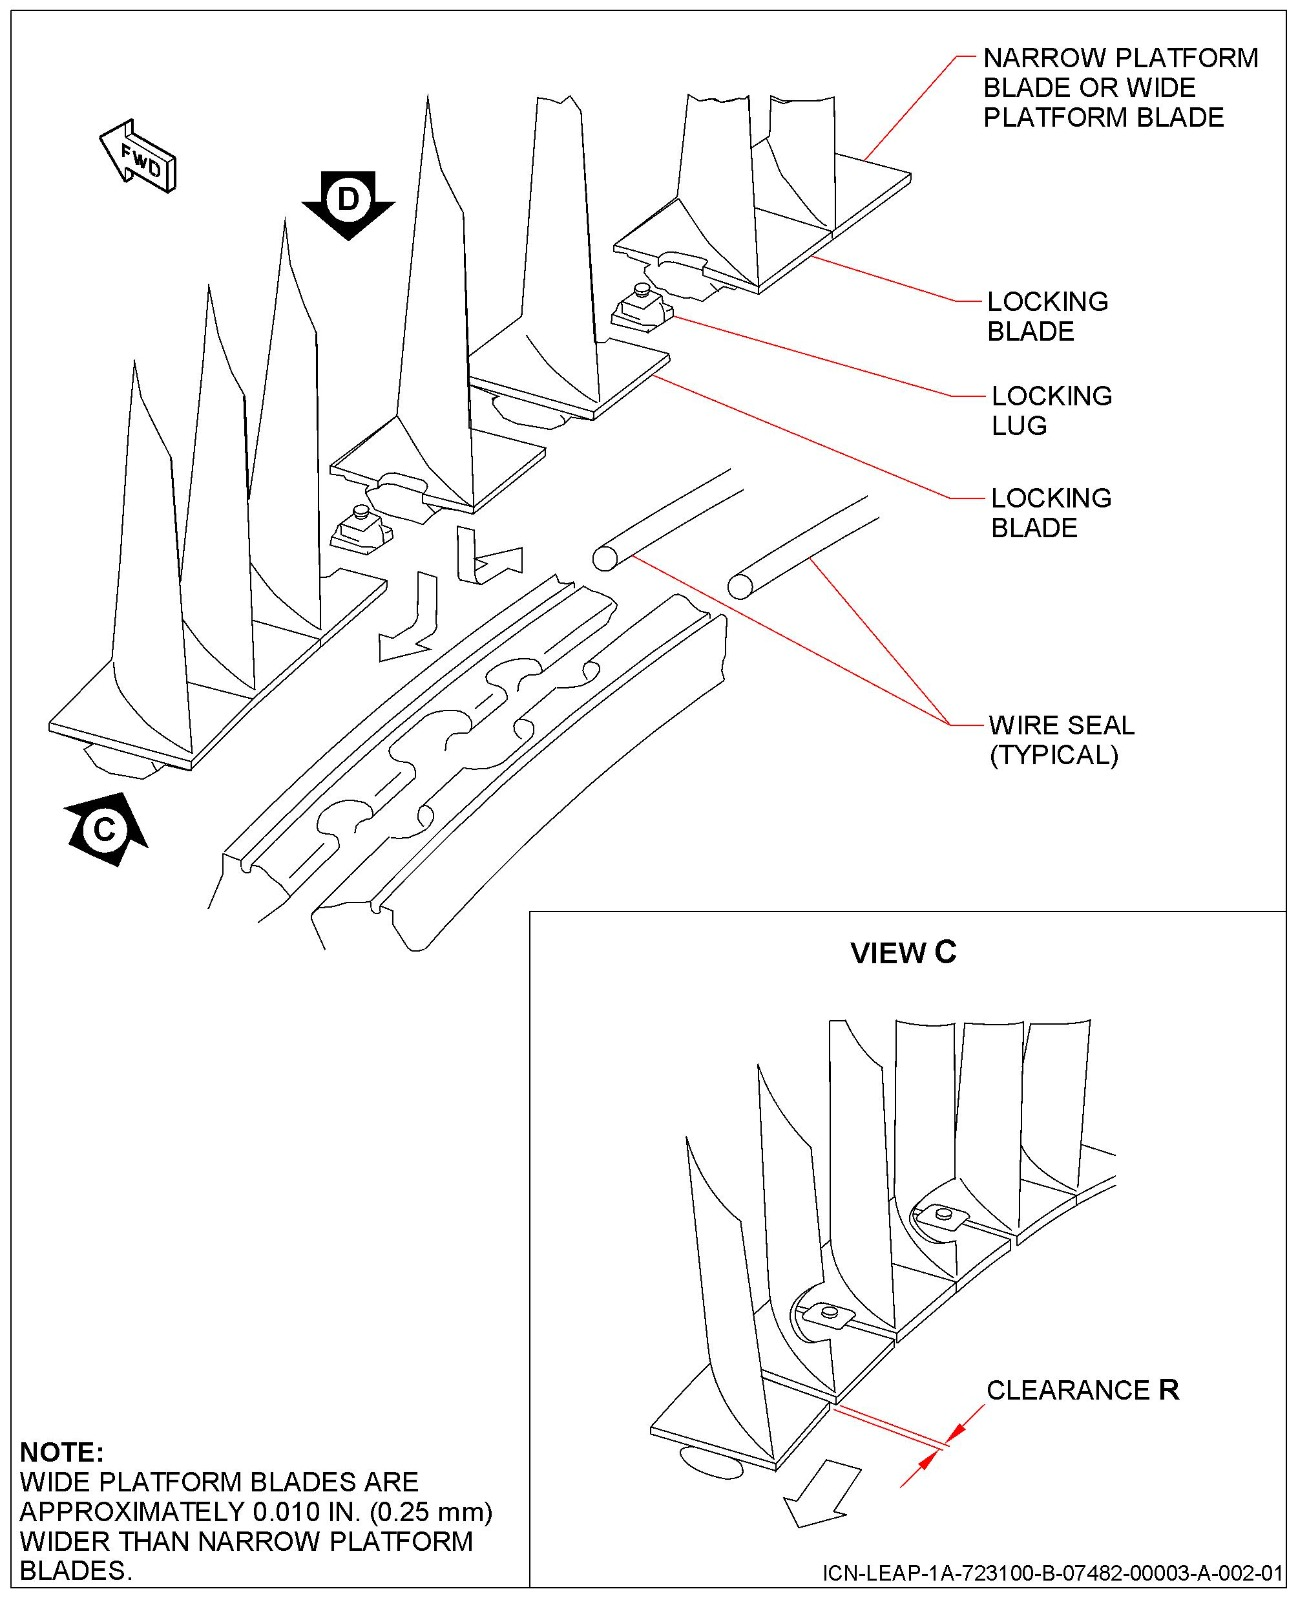
\includegraphics[width=0.5\textwidth]{assembly6.jpeg}
    \caption{Stage Components and Clearence Representation}
    \label{fig:assembly6}
\end{figure}


The measurement of the clearance is performed using a feeler gauge (with a corresponding image), ensuring precise determination of the gap. For each compressor stage, a predefined clearance value is specified, as presented in Table~\ref{tab:clearance_tolerance}. In the aviation industry, these clearance values are typically provided in inches. However, throughout the development of this dissertation, all measurements have been converted to millimeters to maintain consistency.

Once the correct blade sequence and clearance are established, the assembly is reinstalled, and a final torque check is performed on the locking lugs. Ensuring that all components remain within the prescribed limits is critical to maintaining engine performance and durability, as deviations from the specified tolerances can lead to excessive wear, unwanted vibrations, or mechanical failures.

\begin{table}[h]
    \centering
    \begin{tabular}{ccccc}
        \toprule
        Stage & \makecell{Assembly Clearance \\ Tolerance [in]} & \makecell{Assembly Clearance \\ Tolerance [mm]} & Clearance [mm]\\
        \midrule
        6  & 0.010-0.030 & 0.254-0.762  &  \\
        7  & 0.010-0.030 & 0.254-0.762  &  \\
        8  & 0.010-0.030 & 0.254-0.762  & 0.508 \\
        9  & 0.080-0.100 & 2.032-2.54   &   \\
        10 & 0.149-0.169 & 3.7846-4.2926 &  \\
        \midrule
    \end{tabular}
    \caption{Assembly clearance tolerances for different stages.}
    \label{tab:clearance_tolerance}
\end{table}

Currently, in \gls{TAP}'s \gls{ME} Engine Shop assembly process, there is no method to anticipate this clearance before the assembly stage. As a result, if the measured clearance after assembly does not fall within the required specifications, additional wide-platform blades may need to be sourced from the supplier. This can introduce delays in the workflow, as the availability of the necessary blades depends on supplier lead times. As represented in Figure~\ref{fig:assembly6}, wide-platform blades are approximately 0.25 mm wider than narrow blades, allowing for clearance adjustments when needed. Implementing a way to predict and control clearance earlier in the process would help streamline operations, reducing waiting times and improving overall efficiency.

As a first step, it is necessary to construct a nominal model of the blades from which further work can be carried out. This model will serve as the foundation for predicting and controlling assembly clearances, ensuring compliance with specifications, and improving process efficiency.

\subsection{Measurement Challenges and Limitations}
\label{subsec:desafios}

One of the primary challenges in ensuring proper assembly clearance is the precision required to construct a nominal model of the blades. The assembly clearance depends on the individual blade dimensions, particularly the platform width, as these factor determine how the blades fit within the spool slots. To develop an effective process, it is essential to establish a nominal blade model with a precision level derived from the permissible clearance tolerances.

The required precision level can be derived from the assembly clearance by considering the maximum allowable variation that still maintains compliance. This ensures that the model reflects real-world manufacturing conditions and enables accurate clearance prediction.

To define the tolerance for the nominal model, a statistical approach is utilized, as described in \cite{TSM}. Unlike the total interchangeability model, where tolerances are summed linearly, the statistical model considers the probability distribution of component variations. The assembly tolerance is calculated using the following equation:

\begin{equation}
    T_{\text{conj}} = \sqrt{\sum_{i=1}^{n} t_i^2}
    \label{eq:estat}
\end{equation}

where:
\begin{itemize}
\item $T_{\text{conj}}$ - Assembly Tolerance
\item $t_i$ - Part Tolerance
\end{itemize}

This approach reduces the overall tolerance accumulation, making it more suitable for large-scale production where component variations follow a normal distribution. By applying this model, it is possible to maintain a precise nominal blade model while accommodating natural manufacturing variations.

\subsection{Calculation of Platform Dimensional Tolerance for Each Blade Type and Stage}
\label{subsec:clearance_calculation}
To evaluate the dimensional tolerance for each compressor stage, the number of wide and narrow blades assembled in the engine was analyzed. Table~\ref{tab:blade_distribution} presents the distribution of wide and narrow blades for each stage, along with the total number of blades.
The assembly data was collected from a motor assembled in the workshop to determine the exact number of blades used.
\begin{table}[h]
    \centering
    \begin{tabular}{@{}cccc@{}}
        \toprule
        Stage & Wide Blades & Narrow Blades & Total Blades \\ 
        \midrule
        6  & 26 & 36 & 62 \\ 
        7  & 24 & 33 & 57 \\ 
        8  & 24 & 39 & 63 \\ 
        9  & 23 & 37 & 60 \\ 
        10 & 26 & 39 & 65 \\ 
        \bottomrule
    \end{tabular}
    \caption{Number of wide and narrow blades per stage.}
    \label{tab:blade_distribution}
\end{table}

Using the equation \ref{eq:estat}, and considering an assembly tolerance of 0.508 mm, we analyze the case for stage 6, which has 26 wide blades and 36 narrow blades. Beign almost identical parts, its assumed that the wide body and narrow body blades present the same tolerance, \( T_w = T_n \), the equation simplifies to:

\begin{equation}
    T_{\text{conj}} = \sqrt{26T_w^2 + 36T_n^2}
\end{equation}

\begin{equation}
    T_{\text{conj}} = \sqrt{62T_w^2} = \sqrt{62} T_w
\end{equation}

Since the total assembly tolerance is given as 0.508 mm:

\begin{equation}
    0.508 = \sqrt{62} T_w
\end{equation}

Solving for \( T_w \):

\begin{equation}
    T_w = \frac{0.508}{\sqrt{62}} = 0.0646 \text{ mm}
\end{equation}

Thus, the tolerance for each blade in stage 6 is approximately **0.0646 mm**.

Based on this analysis, the clearance values were calculated. Table~\ref{tab:clearance} presents the obtained results.

\begin{table}[h]
    \centering
    \begin{tabular}{@{}ccc@{}}
        \toprule
        Stage & Clearance (mm) & Tw = Tn \\ 
        \midrule
        6  & & 0,064516065    \\ 
        7  &   & 0,067286244    \\ 
        8  & 0.508  & 0.00000 \\ 
        9  &   & 0,065582518    \\ 
        10 &   & 0,063009645    \\ 
        \bottomrule
    \end{tabular}
    \caption{Computed clearance values per stage.}
    \label{tab:clearance}
\end{table}

These calculations, derived from workshop data and statistical analysis, ensure that the clearance assessment aligns with real assembly conditions. Furthermore, they provide insight into the required precision needed to develop a nominal model that enables a feasible and applicable solution.

Following this analysis, the next steps involve evaluating the available equipment previously mentioned in \ref{cha:lorem_ipsum}, specifically the Creaform HandySCAN 3D scanner and the Mitutoyo Euro-C 121210 \gls{CMM}. While the application of reverse engineering using the scanner enables the creation of a model, its lower accuracy on edges may compromise the precision required to resolve the problem. Therefore, it is necessary to use the CMM to obtain the geometry with the required accuracy. Additionally, the scanner enables the development of the CMM fixture, which will be designed using knowledge from previous dissertations.

The accuracy of the available equipment is as follows:  

\begin{itemize}
    \item HandyScan accuracy: 0.001 in (0.0254 mm)
    \item Peripheral tape accuracy: 0.0005 in (0.0127 mm)
    \item CMM accuracy: 0.00001 in (0.00000254 mm)
\end{itemize}

These values highlight the significant difference in measurement precision, reinforcing the need for a combined approach to achieve the required accuracy.

\subsection{Spool Measurements and Specifications}
\label{subsec:spool_measurements}

To ensure precise assembly and proper clearance for the HPC blades, it is essential to define the key dimensions of the spool. The spool serves as the foundational structure for blade installation, and its dimensions directly impact the assembly process. Table~\ref{tab:spool_dimensions} presents the main geometric characteristics of the spool relevant to the blade assembly process.


\begin{figure}[H]
    \centering
    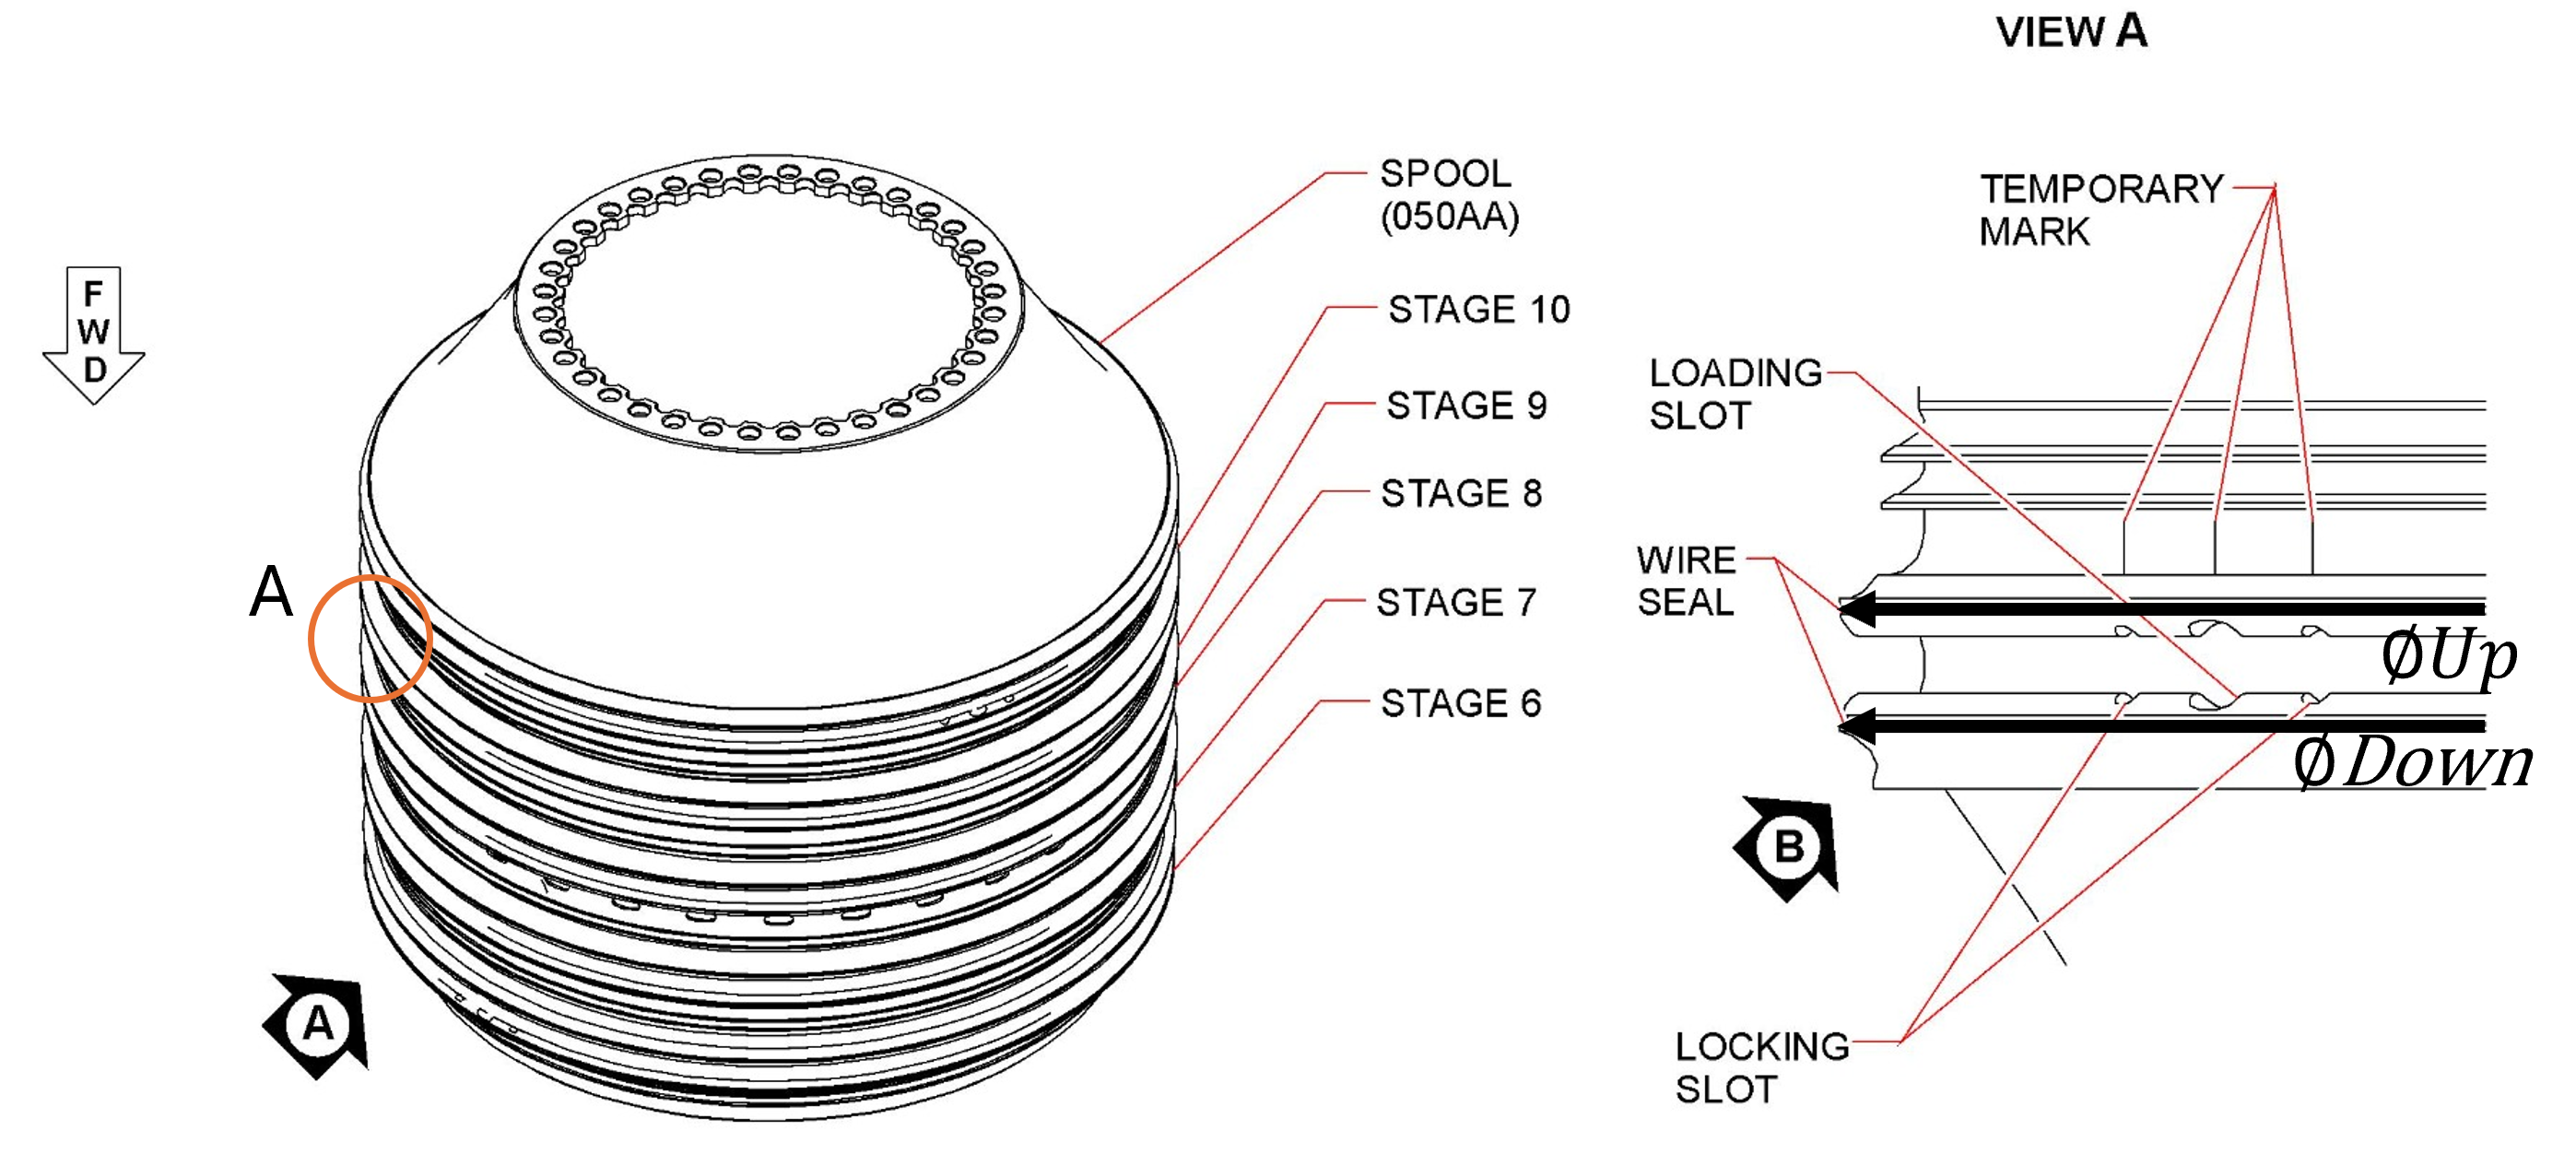
\includegraphics[width=0.8\textwidth]{diam.png}
    \caption{Stage Components and Clearence Representation}
    \label{fig:diam.png}
\end{figure}

\begin{table}[h]
    \centering
    \begin{tabular}{|c|c|c|}
        \hline
        Stage & ØUp & ØDown \\
        \hline
        10 & 15.675 & 15.69 \\
        9  & 15.704 & 15.66 \\
        8  & 15.670 & 15.62 \\
        7  & 15.620 & 15.69 \\
        6  & 15.545 & 15.52 \\
        \hline
    \end{tabular}
    \caption{Diameter values for each stage}
    \label{tab:diameters}
\end{table}


These dimensions play a crucial role in determining the fit and function of the HPC blades. The slot width and depth directly influence how securely the blades are held in place, while the groove width and depth are vital for the proper installation of wire seals. Additionally, platform clearance values dictate the permissible gap between adjacent blades, ensuring compliance with operational specifications.

By integrating these spool measurements into the assembly process analysis, it is possible to predict and optimize the blade fitting conditions before final assembly, reducing rework and improving overall efficiency.



\chapter{Design and Application of Tooling for CMM: Scanning, Point Cloud Processing, and Fixation System Modeling}
\label{cha:digi}

\section{Introduction}
\label{sec:intro2}


\section{Scanning of the Blades}
\label{sec:scan}

programa utilizado no scan, tratamento 
falar da falha no scan e dificuldade nas edges

\section{Point Cloud Processing and CAD Model Creation}
\label{sec:cad}

xtract3d 
Consideraçoes


\chapter{Design and Application of Tooling for CMM: Scanning, Point Cloud Processing, and Fixation System Modeling}
\label{cha:dig}










